\chapter{Geometric Set Cover with segments}

\section{FPT for segments}
\subsection{Segments parallel to one of the axis}
You can find this in Platypus book.

We'll show $\mathcal{O}(2^k)$ branching algorithm.
Let's take point $K$ that hasn't been covered yet with
the smallest coordinate in lexicograpical order.
We need to cover $K$ with some of the remaining segments.

We choose one of the 2 directions on which we will cover this point.
In this direction we take greedly the segment that will cover
the most points (there are points in $\points$ only on
one side of $K$ in this direction, so all
segments covering $K$ in this direction create monotone sequence
of sets -- zbiory zstępujące).

\subsection{Segments in $d$ directions}
The same algorithm as before but in complexity $\mathcal{O}(d^k)$.

\subsection{Segments in arbitrary direction}
\begin{tw}{
	\textbf{(FPT for segment cover)}.
	There exists an algorithm that given a family $\sets$ of
	$n$ segments (in any direction),
	a set of $m$ points $\points$
	and a parameter $k$,
	runs in time $f(k) \cdot (nm)^c$ for some computable function f and constant c,
	and outputs a subfamily $\sol \subseteq \sets$
	such that $|\sol| \le k$ and $\sol$ covers all points in $\points$.
}\end{tw}
\paragraph{Proof.}
We will show such algorithm in FPT.

If there exist two segments $a$ and $b$ in $\sets$,
such that any point covered by $a$ is also covered by $b$,
then without loss of generality we can remove segment $a$ from $\sets$.
We repeat this process until no such $(a, b)$ pair exists.


Let us first assume that we reduced our instance to a kernel,
where \textit{any line} contains no more than $k$ points.

Since any segment covers a set of colinear points,
for such a kernel $k$ segments can cover only at most $k^2$ points.
Therefore, for the answer to be positive,
the number of points has to be at most $k^2$.
The number of segments is now bounded by $k^4$,
since if we consider two \textit{extreme} points
covered by a given segment,
then these pairs must be distinct,
otherwise two segments would contain the same set of points.
Since both the number of points and the number of segments
is bounded by a function of $k$,
this instance can be easily solved in time $O(f(k))$.

In remains to show how to construct the kernel.

%As long as there is a line with more than $k$ points, do branching.
%Let's name points on this line $x_1, x_2, \ldots x_t$
%in order they appear on the line.

%So we choose on which point the chosen segment on this line
%will start. Of course we have to take at least one segment
%covering at least one point among first $k+1$ points,
%because covering all of them with only segments
%on different lines we would use
%exactly $k+1$ segments (any of them can't contain more than
%one point from this line).


Assume there exists a line $l$ containing points $x_1$, \ldots $x_t$,
where $t \geq k + 1$.
Note that a segment that does not lie on $l$ can cover only at most one
of the points $x_i$.
Therefore, out of points $x_1$, ..., $x_{k+1}$,
at least one has to be covered by a segment that lies on $l$,
let us fix $x_i$ to be the first such point.
Then, we can greedily choose a segment that lies on $l$,
covers $x_i$,
and also covers the largest number of points $x_j$ for $j > i$.

Since we have at most $k + 1$ choices to branch over
and each choice adds a segment to the constructed solution,
we obtain an algorithm with complexity $O(k^k)$.

\section{APX-completeness for segments parallel to axis}
\label{section:segment_apx}

\begin{tw}{
	Given an instance of unweighted geometric set cover
	with axis-parallel segments in 2D and $\epsilon>0$, there doesn't
	exist $(1+\epsilon)$-approximation scheme unless $ETH$ fails.
}\end{tw}

It works even with extensions for unit weights.

We will show reduction from MAX-(3,3)-SAT
to Geometric Set Cover with segments pararell to axis.

\subsection{Definition of  MAX-(3,3)-SAT problem}
Here we define MAXSAT problem.

\subsection{Reduction construction}

Let's take some instance of  MAX-(3,3)-SAT with
variables $x_1, x_2 \ldots x_n$
and clauses $C_1, C_2 \dots C_n$.

We will create gadgets for choosing the value
of variables (\textit{true} or \textit{false}) and checking
if the clauses are met (any of the variables were chosen).

\begin{figure}[h]
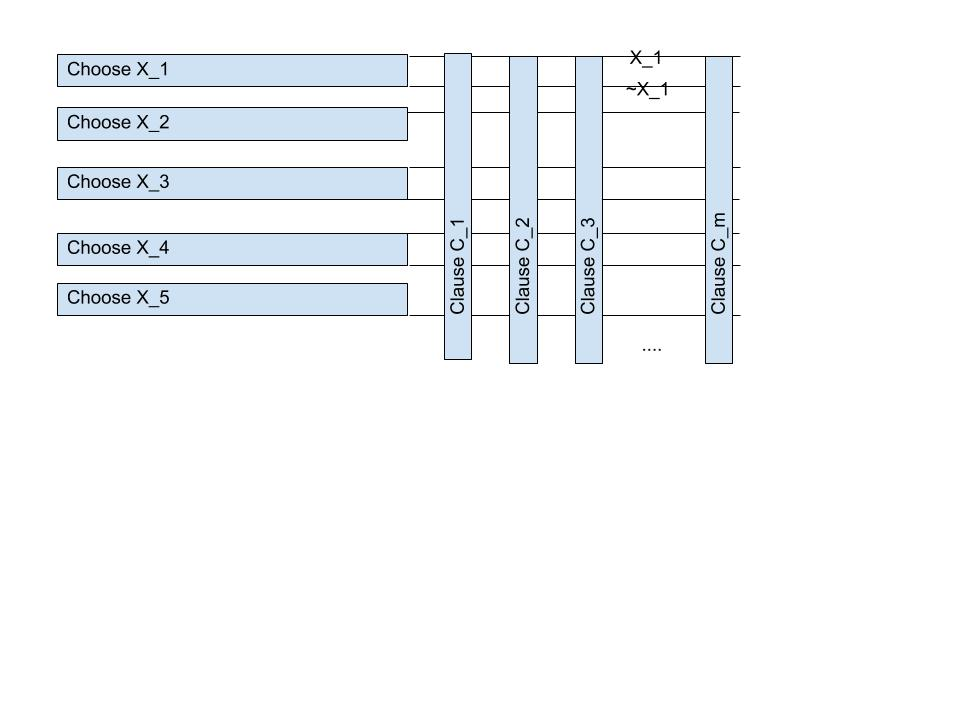
\includegraphics[width=0.7\textwidth]{segment_apx_sketch.jpg}
\caption{General scheme of reduction.}
\label{fig:segment_apx}
\end{figure}

\subsubsection{Choose $x_i$ gadget}
\begin{figure}[h]
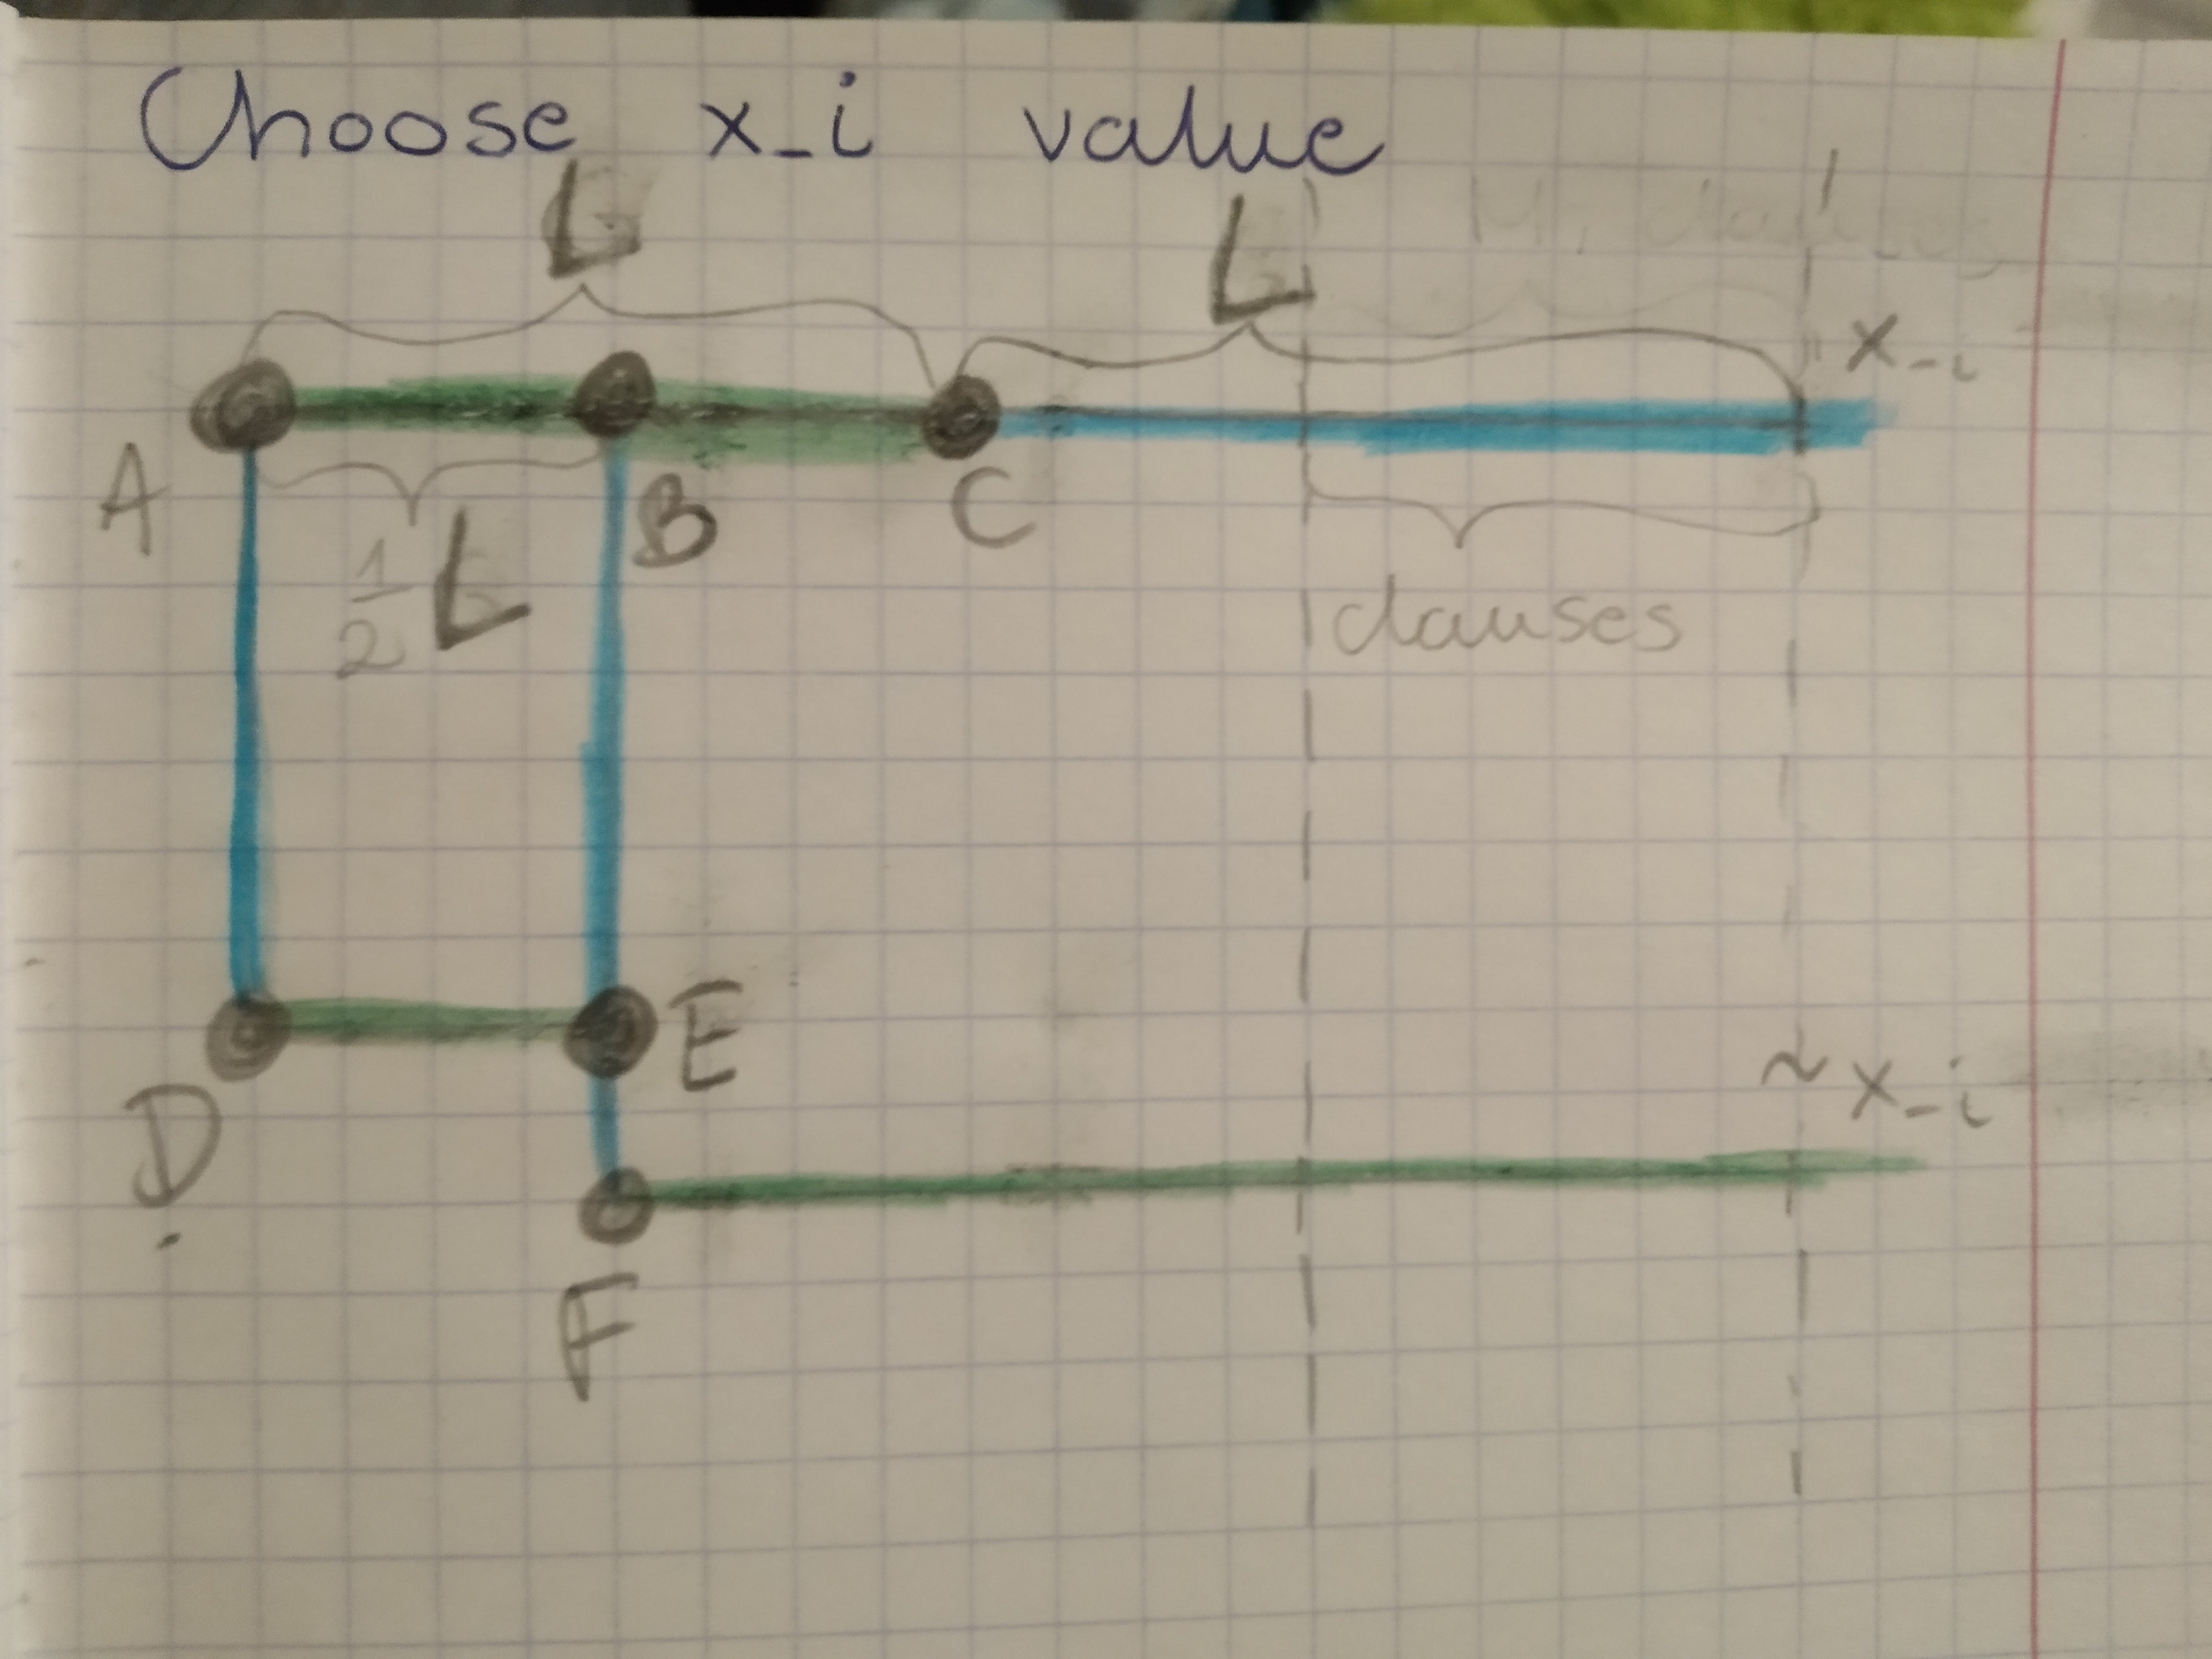
\includegraphics[width=0.6\textwidth]{choose_x_gadget.jpg}
\caption{Scheme of choose $x_i$ gadget.}
\label{fig:choose_x_gadget}
\end{figure}
In Figure~\ref{fig:choose_x_gadget},
we show a gadget that simulates a single variable $x_i$.
It consists of six points A, B, C, D, E, F, and several segments.
Selecting the segment marked with $x_i$
to the solution will correspond to setting $x_i$ to \textit{true},
while selecting the segment marked with $\neg x_i$
to setting $x_i$ to \textit{false}.
In the following lemmas,
we show that this construction indeed models a binary variable.

First, note that in the gadget
there are exactly two sets of three segments
that cover all points $A, B, C, D, E, F$.
These two sets of segments are marked in
Figure~\ref{fig:choose_x_gadget} in blue and green, respectively.

\begin{lemma}
Points $A, B, C, D, E, F$ cannot be covered using less than
3 segments (even with $1/2$-extensions).
\end{lemma}
\paragraph{Proof.}
We need to take at least one segment on line $ABC$,
because it's the only way to cover $C$.
All other points ($D, E, F$) are not colinear,
so we need at least 2 other segments to cover them.

\begin{lemma}
If we choose both segments $x_i$ and $\neg x_i$, we need to use at
least 4 segments to cover all points $A, B, C, D, E, F$
(even with $1/2$-extensions).
\end{lemma}

\paragraph{Proof.}
Choosing both segments $x_i$ and $\neg x_i$
we only cover points $C$
(becuase $B$ is too far away to be covered with $1/2$-extension)
and $F$.

The remaining points ($A, B, D, E$) are not colinear,
so we need at least two more segments to cover them.

\paragraph{Robustness to $1/2$-extension.}
Take a look at Figure~\ref{fig:segment_apx}.
The points will be included in choose gadgets (horizontal boxes)
and clause gadgets (vertical boxes).

Since segment $AC$ is very long
and colinear with $x_i$, after $1/2$-extension
it will cover a significant part of segment $x_i$,
even though $x_i$ will not be chosen.

If we put all the clause gadgets in the area
marked with \textbf{clauses} at gadget scheme in Figure~\ref{fig:choose_x_gadget},
it is enough to prove that $AC$ will not cover any points
in the \textbf{clauses} area even with $1/2$-extensions.

\begin{lemma}
No points in \textbf{clauses} area can be covered
by $AC$ with $1/2$-extension.
\end{lemma}

\paragraph{Proof.}
Bear in mind that length of $AC$ is equal to length of $x_i$.
Area \textbf{clauses} takes a second half
of the segment $x_i$ and $AC$ after extension will cover the first
half of segment $x_i$.

\subsubsection{Clause gadget}
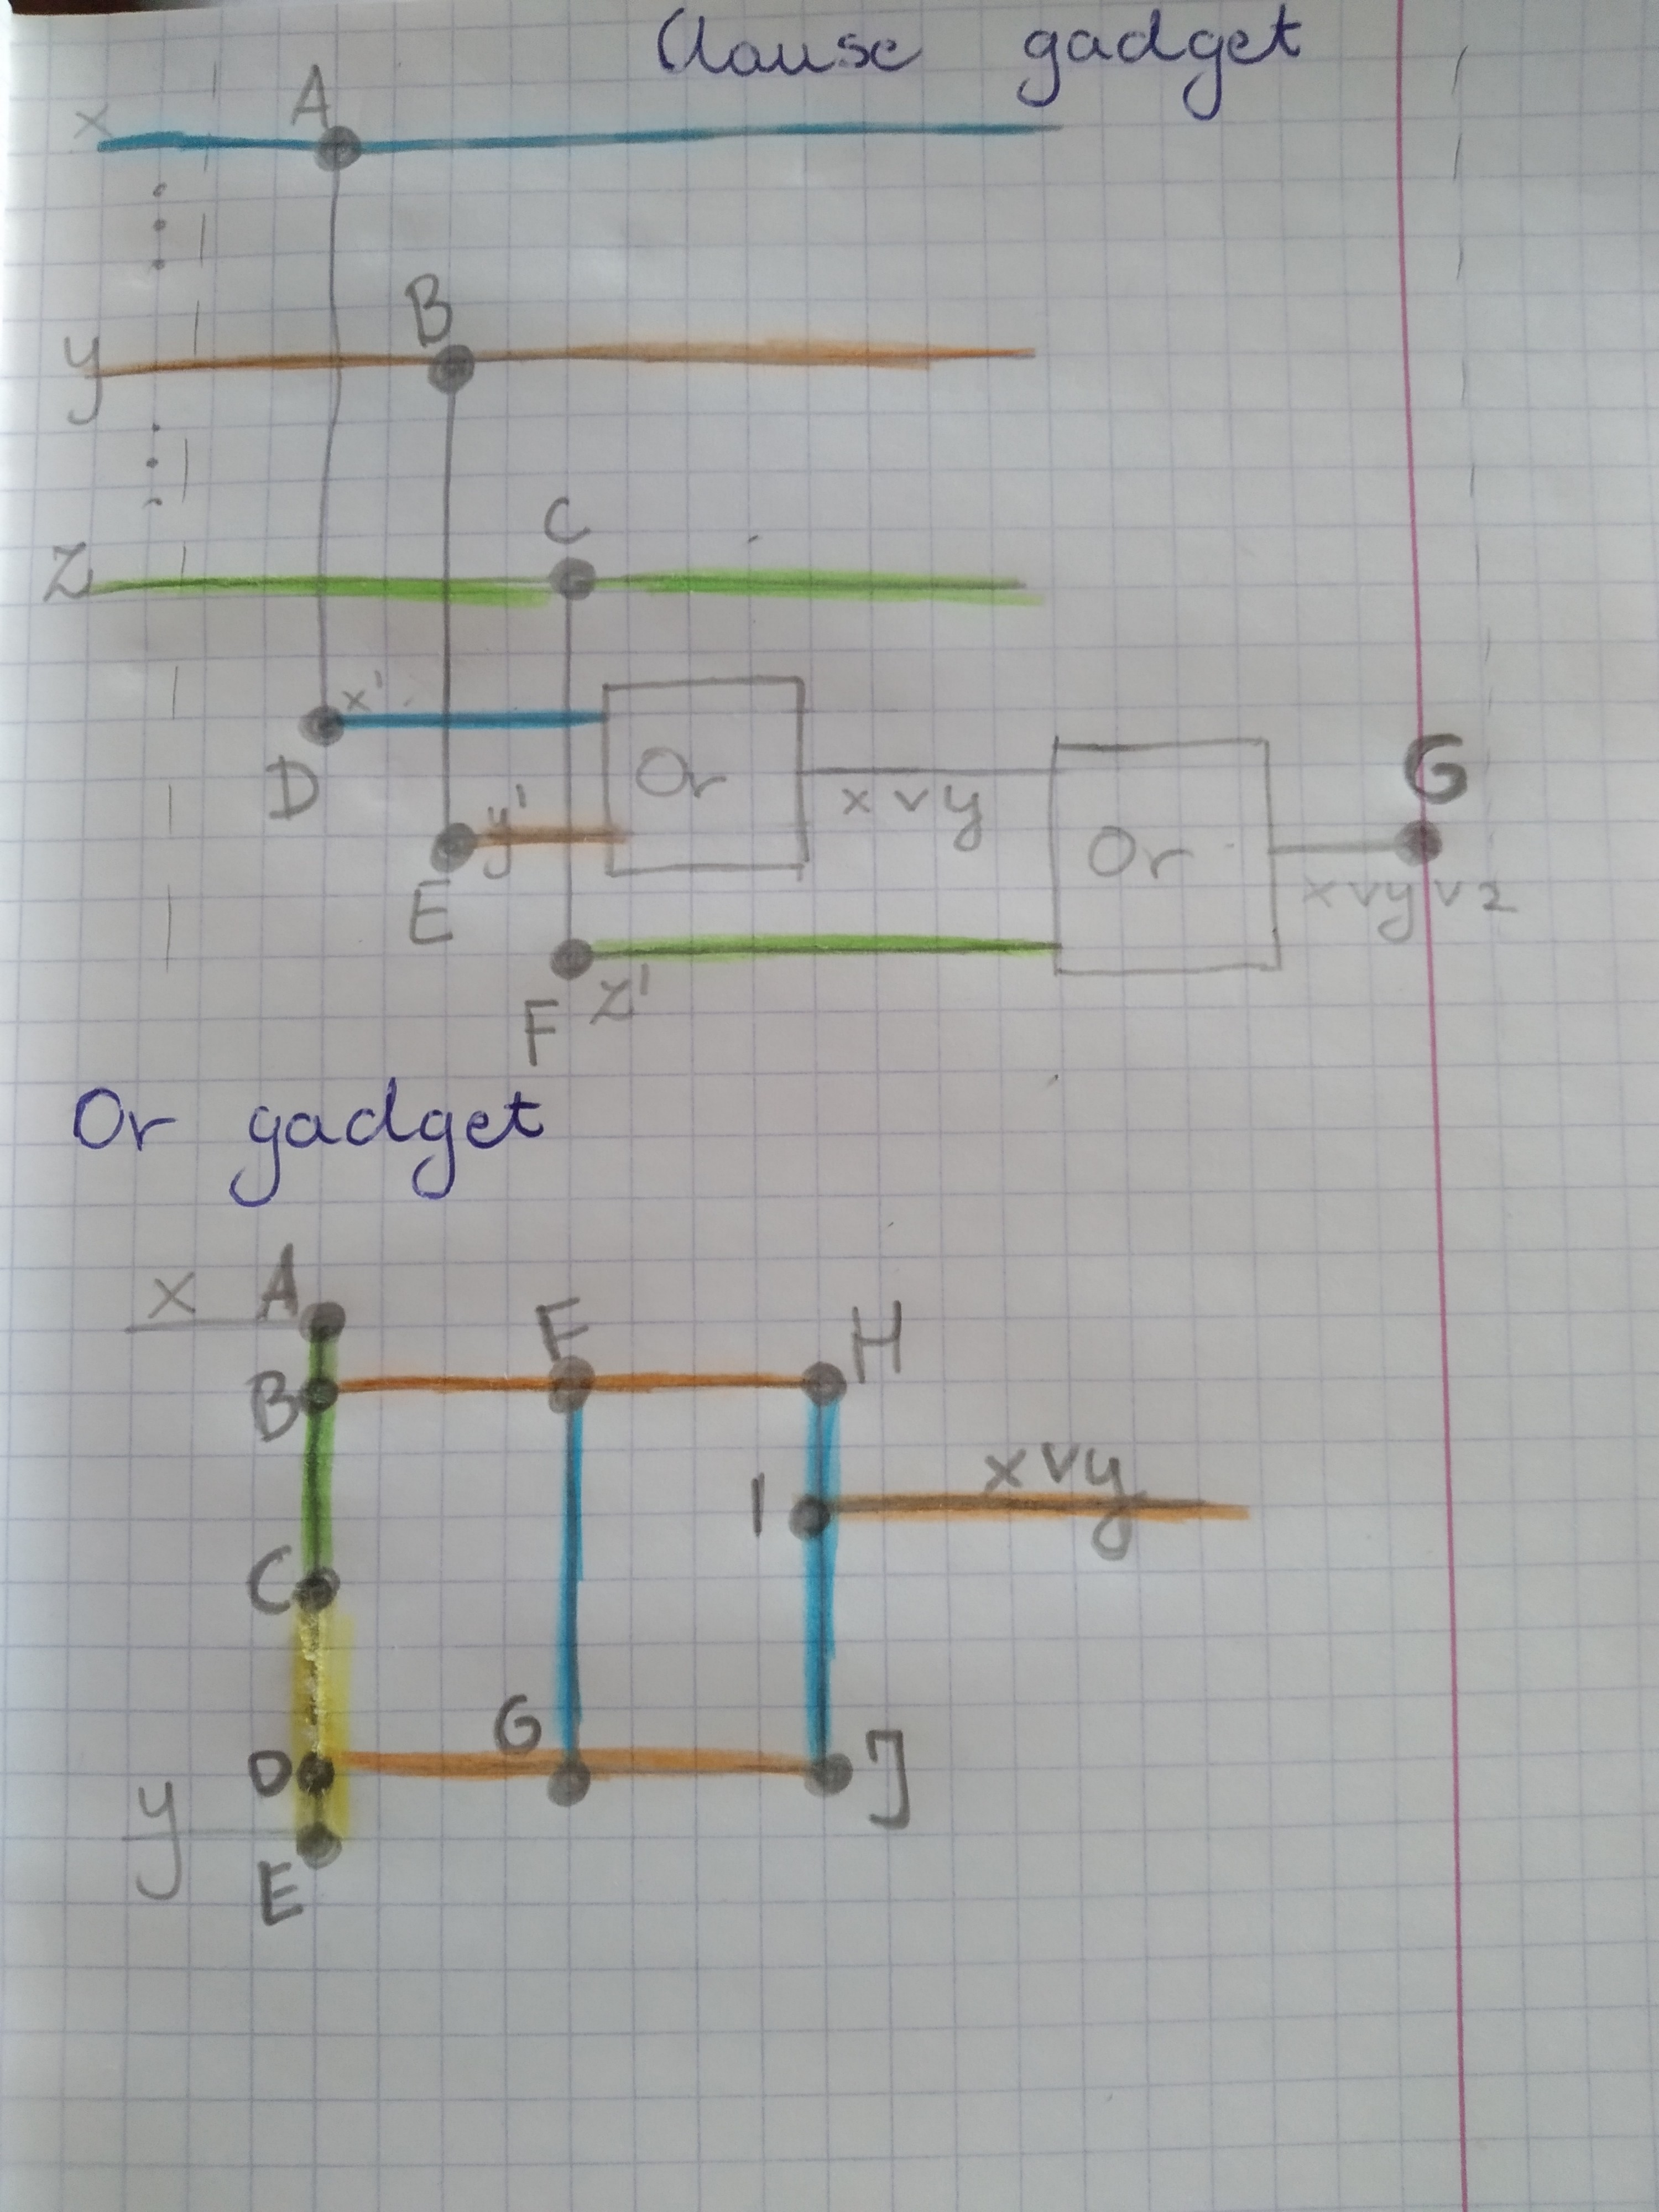
\includegraphics[width=0.6\textwidth]{clause_gadget.jpg}

\begin{lemma}
In order to cover $D$ ($E, F$) point at least one
of the segments $AD$ ($BE, CF$) or $x'$ ($y', z'$).
\end{lemma}

\begin{lemma}
Points $A$ and $D$ can be covered
with one additional segment $x'$
only if $x$ is already chosen.
Otherwise they can be covered with one segment
only by using $AD$.
\end{lemma}

\begin{lemma}
Points $A, B, C, D, E, F, G$ can be covered with 
3 or 4 segments, depending if at least one of the segments
$x, y, z$ was previously chosen.
\end{lemma}

\subsubsection{Or gadget}
\begin{lemma}
Points $A, B, C, D, E, F, G, H, I, J$ can be covered using
at least 4 segments even with $1/2$-extension.
\end{lemma}

\begin{lemma}
Points $A, B, C, D, E, F, G, H, I, J$ can be covered using
4 segments and segment $x \lor y$ can be chosen
even with $1/2$-extension
only if at least one of the segments $x$ or $y$ is chosen.
\end{lemma}

\subsection{Proof that construction is sound}
\begin{lemma}
If there exists setting of values of variables that exactly $k$
clauses are satisfied, we can cover all the points
with $3n + 11m + (m-k)$ segments.
\end{lemma}

\begin{lemma}
If there exists cover with $k$ segments,
then also there exists solution for MAX-(3,3)-SAT.

TODO: Formulate this lemma better.
\end{lemma}

\section{Weights}
\subsection{FPT for segments pararell with $\delta$-extensios}
\subsection{W[1]-completeness for arbitrary segments with weights}
\subsection{What is missing}
We don't know FPT for pararell segments
and arbitrary lines with $\delta$-extensions.
